% !TeX encoding = UTF-8
% !TeX root = RosNavTuningCn.tex
% !TeX TS-program = xelatex.exe


\section[Velocity and Acceleration]{速度和加速度}
本节涉及同步驱动(synchro-drive)机器人。机器人的动力学特征(例如,机器人的速度和加速度)对于动态窗口法(Dynamic Window Approach, DWA)和定时弹性带(Timed Elastic Band, TEB)这两种局部规划器是必不可少的内容。
在ROS的导航功能包中,局部规划器接收里程消息(“\mintinline{bash}{odom}"话题),输出控制机器人运动的速度指令(“\mintinline{bash}{cmd_vel}”话题)。

速度和加速度的最大/最小值是移动基座的两个基本参数。
正确设置这两个数值对优化局部规划器的移动行为帮助非常大。
在ROS的导航中,我们需要知道平移和旋转的速度及加速度。	


\subsection[To obtain maximum velocity]{获取最大速度}
一般可以参考你的移动基座的手册。例如,SCITOS G5的最大速度为1.4 m$/$s\footnote{此信息来自于\href{http://www.metralabs.com/en/research}{MetraLabs网站}。}。
在ROS中,你还可以订阅\mintinline{bash}{odom}话题以获取当前里程信息。如果你能手工控制机器人(例如使用操纵杆),则你可以尝试向前移动直到它的速度值达到常数,
然后回显(echo)里程数据。

\textit{平移速度}($m/s$)是机器人沿直线移动时的速度。获取其最大值的方式与上面获取最大速度的方式相同。\textit{旋转速度}($rad/s$)等效于角速度;它的最大值是机器人在原地位置旋转时的角速度。为获取最大旋转速度,我们可以通过操纵杆控制机器人,在机器人的速度达到恒定值后将机器人旋转360度,并对此次运动进行计时。

为安全起见,我们倾向于将最大平移速度和旋转速度设置为低于其实际最大值。	




\subsection[To obtain maximum acceleration]{获取最大加速度}

若您的手册没有直接告诉您该值大小,可通过很多方法测量您的移动基座的最大加速度。

在ROS中,类似地,我们可以回显包含时间戳的里程数据,记下机器人达到最大平移速度时所花的时间($t_{i}$)。
之后我们利用里程计的位置和速度信息(\mintinline{bash}{nav_msgs/Odometry}消息)计算此过程中的加速度。
多做几条不同的路径,计算其平均值。
分别用$t_t$和$t_r$表示机器人从静止达到最大平移速度和最大旋转速度所需要的时间。
则最大平移加速度为$a_{t,max}=\text{max }dv / dt\approx v_{max}/t_t$。
同理,最大旋转加速度通过式$a_{r,max}=\text{max }d\omega / dt\approx \omega_{max}/t_r$计算。

\subsection[Setting minimum values]{设置最小值}

设置最小速度不必像上述公式那么正式。 
对于最小平移速度,我们希望将其设置为较大的负值,
因为这样可以让机器人在需要自救时进行回退,虽然在大多数实际情况下它应该前进。
对于最小旋转速度,我们希望将其设置为负值(若参数允许的情况下),以便机器人可以在任一方向上旋转。 
注意,DWA局部规划器采用的是机器人最小旋转速度的绝对值。


\subsection[Velocity in x, y direction]{x,y方向上的速度}

{$x$}-\emph{速度}表示平行于机器人直线运动方向的速度。它与平移速度相同。
$y$-\emph{速度}是垂直于该直线运动方向的速度。
在\mintinline{bash}{teb_local_planner}中称为“扫射速度”(strafing velocity)。
对于\emph{非完整类型}(non-holonomic)的机器人(例如差动轮式机器人),应将$y$-\emph{速度}设置为零。




\section[Global Planner]{全局规划器}

\subsection[Global Planner Selection]{全局规划器的选择}
要在导航堆栈中使用\mintinline{bash}{move_base}节点,需要配置一个全局规划器和一个局部规划器。ROS有三个全局规划器继承自\mintinline{bash}{nav_core::BaseGlobalPlanner}接口:\mintinline{bash}{carrot_planner},\mintinline{bash}{navfn}和\mintinline{bash}{global_planner}。

\subsubsection{carrot\_planner}

这是最简单的全局规划器。 
它检查给定的目标点是否在障碍区,如果目标点在障碍区,则沿机器人和目标点之间连线,在连线上选择一个最接近原始目标点的有效目标点。 
最终,它将该有效目标点直接传递给局部规划器或内部控制器。
所以,该规划器并没有进行任何的规划。
它在你需要移动机器人到给定目标点而且目标点无法到达的情况下很有用。
在复杂环境下,该规划器并不实用。

\subsubsection[navfn and global\_planner]{navfn 和 global\_planner}

\mintinline{bash}{navfn} 采用 Dijkstra算法在起点和终点之间寻找一条最小代价的路径。
\mintinline{bash}{global_planner}是\mintinline{bash}{navfn}的灵活性替代,提供了更多的选项,包括:
(1) 支持A$*$, (2) 支持二次近似切换, (3) 支持切换风格路径。
\mintinline{bash}{navfn} 和 \mintinline{bash}{global_planner}实现的内容都是基于\cite{brock1999high}的工作。

\subsection[Global Planner Parameters]{全局规划器的参数}

通常情况下我们更喜欢使用\mintinline{bash}{global_planner},现在来看看它的一些关键参数。注意:并非所有的参数都在ROS的官网上罗列出来,但如果你运行rqt动态配置程序时你可以看到它们:
\begin{minted}{bash}
rosrun rqt_reconfigure rqt_reconfigure
\end{minted}
可以让参数\mintinline{bash}{allow_unknown(true)}, \mintinline{bash}{use_dijkstra(true)},  \mintinline{bash}{use_quadratic(true)},  \mintinline{bash}{use_grid_path} \mintinline{bash}{(false)},  \mintinline{bash}{old_navfn_behavior(false)} 保留它们的默认值。
当需要在rviz可视化势力图(potential map)时将\mintinline{bash}{visualize_potential(false)}设置为\mintinline{bash}{true}会带来很多便利。

\begin{figure}[!htb]
	\minipage{0.49\textwidth}
	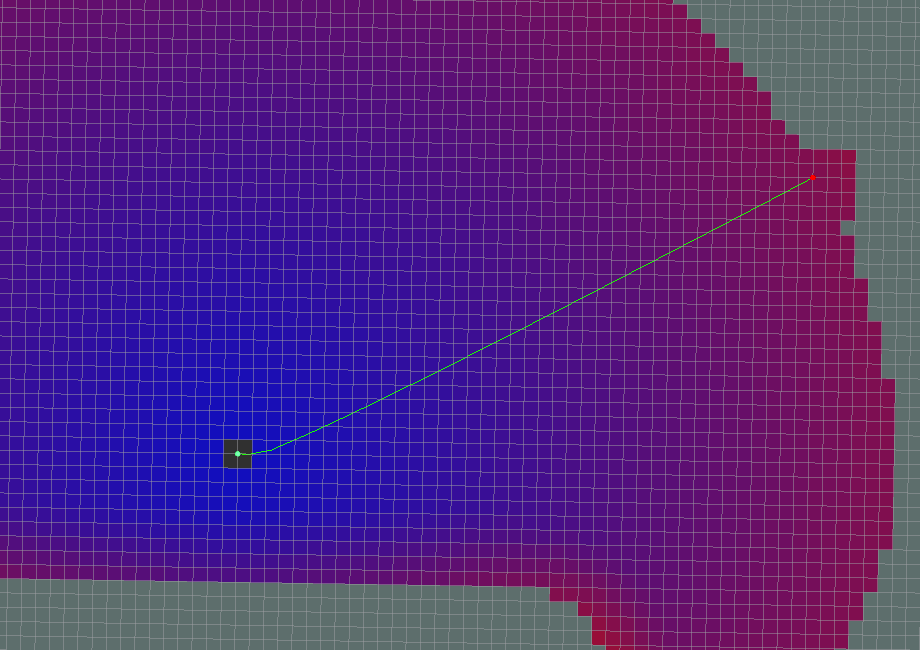
\includegraphics[width=\linewidth]{Dijkstra.png}
	\caption{Dijkstra路径}
	\endminipage\hfill
	\minipage{0.49\textwidth}
	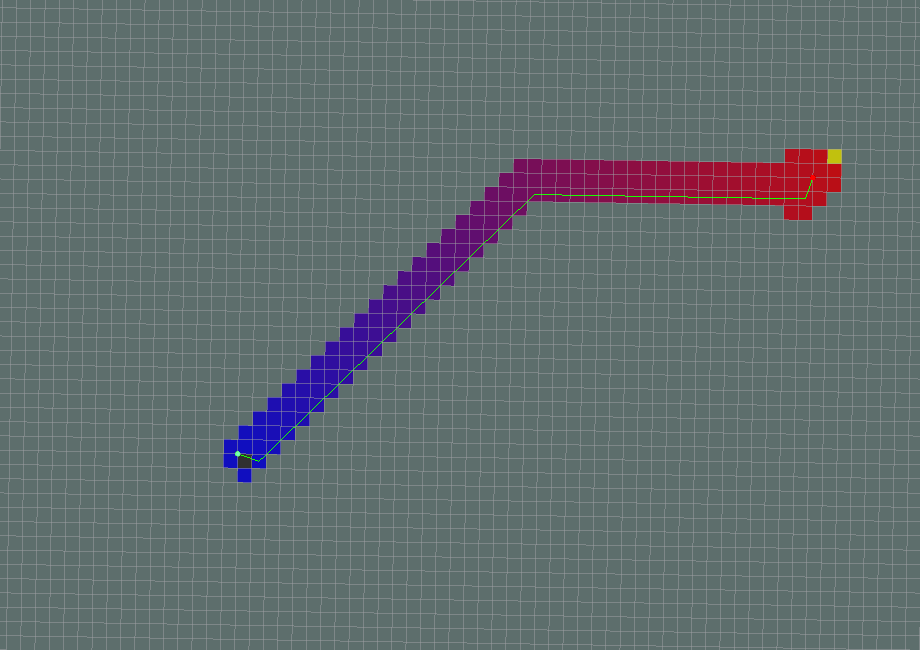
\includegraphics[width=\linewidth]{AStar2.png}
	\caption{A* 路径}
	\endminipage\hfill
\end{figure}

\begin{figure}[!htb]
	\minipage{0.49\textwidth}
	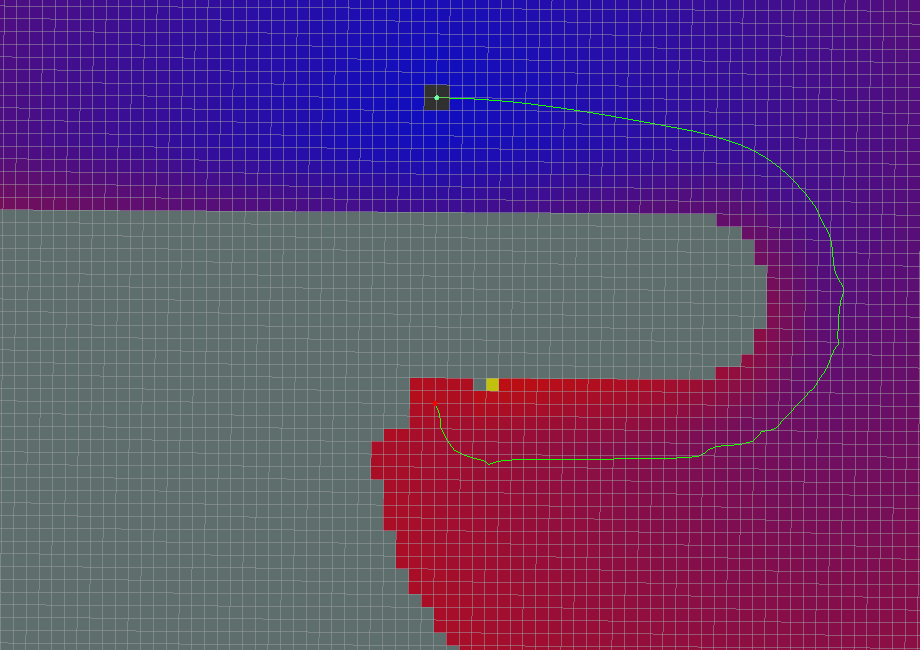
\includegraphics[width=\linewidth]{GlobalPlanner.png}
	\caption{标准行为}
	\endminipage\hfill
	\minipage{0.49\textwidth}
	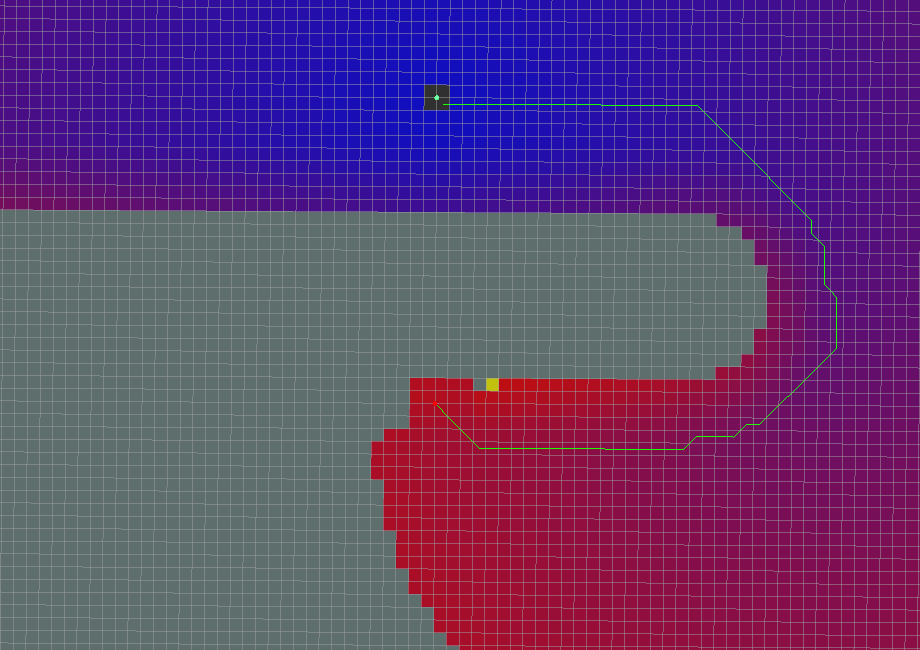
\includegraphics[width=\linewidth]{GridPath.png}
	\caption{网格路径}
	\endminipage\hfill
\end{figure}

除去这三个参数外,还有另外三个未列出的参数对规划全局路径的质量造成很大的影响。它们是\mintinline{bash}{cost_factor}, \mintinline{bash}{neutral_cost}, \mintinline{bash}{lethal_cost}。
实际上,这些参数也存在于\mintinline{bash}{navfn}的配置中。
源程序\footnote{\scriptsize\url{https://github.com/ros-planning/navigation/blob/indigo-devel/navfn/include/navfn/navfn.h}}有一段描述解释了\mintinline{bash}{navfn}是如何计算代价值的。

%\begin{figure}[!htb]
%	\minipage{0.32\textwidth}
%	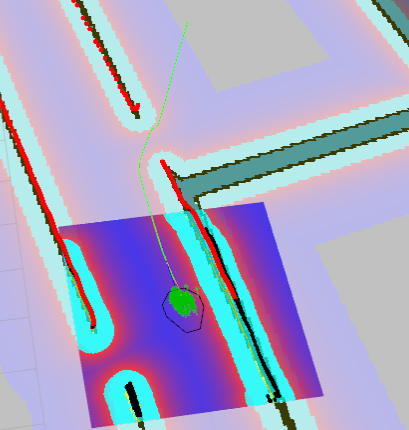
\includegraphics[width=\linewidth]{Cf_lo.png}
%	\caption{\mintinline{bash}{cost_factor} = 0.01}
%	\endminipage\hfill
%	\minipage{0.32\textwidth}
%	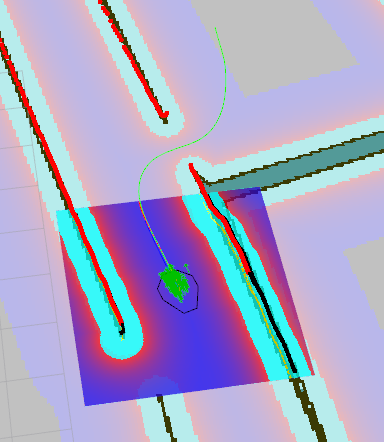
\includegraphics[width=\linewidth]{Cf_mid.png}
%	\caption{\mintinline{bash}{cost_factor} = 0.55}
%	\endminipage\hfill
%	\minipage{0.32\textwidth}
%	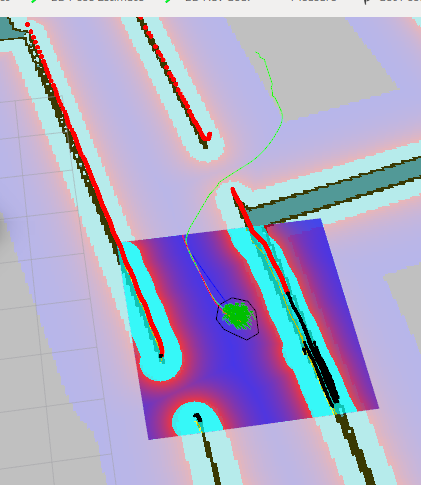
\includegraphics[width=\linewidth]{Cf_hi.png}
%	\caption{\mintinline{bash}{cost_factor} = 3.55}
%	\endminipage\hfill
%\end{figure}

\begin{figure}[!htb]
	\begin{minipage}[t]{0.33\linewidth}
		\centering 
		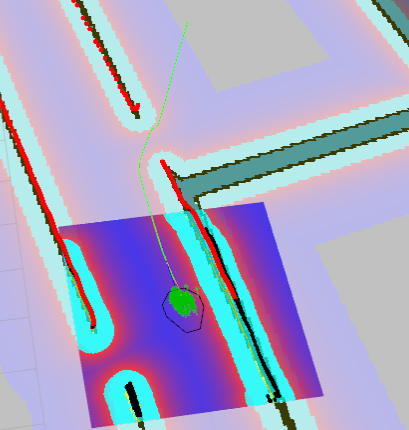
\includegraphics[width=\linewidth]{Cf_lo.png}
		\caption{\mintinline{bash}{cost_factor} = 0.01}
		%\label{fig:side:a} 
	\end{minipage}\hfill
	\begin{minipage}[t]{0.33\linewidth} 
		\centering 
		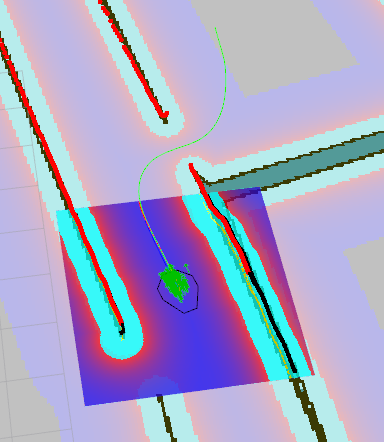
\includegraphics[width=\linewidth]{Cf_mid.png}
		\caption{\mintinline{bash}{cost_factor} = 0.55}
%		\label{fig:side:b} 
	\end{minipage} \hfill
	\begin{minipage}[t]{0.33\linewidth} % 如果一行放2个图,用0.5,如果3个图,用0.33
	 	\centering 
	 	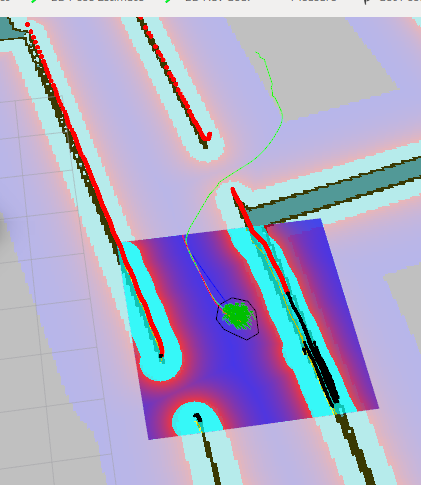
\includegraphics[width=\linewidth]{Cf_hi.png}
	 	\caption{\mintinline{bash}{cost_factor} = 3.55}
%	 	\label{fig:side:a} 
	\end{minipage}\hfill
\end{figure}

%\begin{figure}[!htb]
%	\minipage{0.32\textwidth}
%	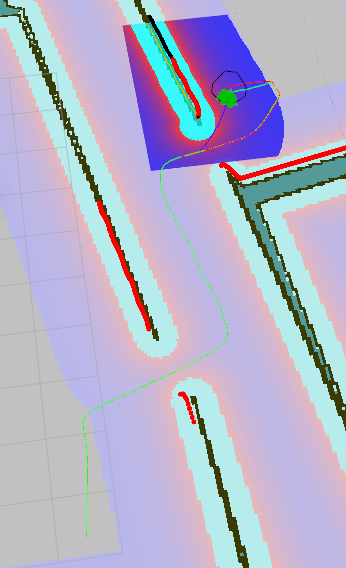
\includegraphics[width=\linewidth]{NC_lo.png}
%	\caption{\mintinline{bash}{neutral_cost} = 1}
%	\endminipage\hfill
%	\minipage{0.32\textwidth}
%	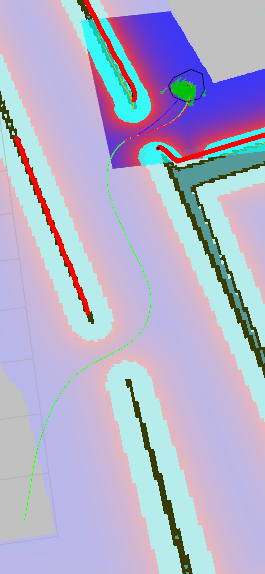
\includegraphics[width=\linewidth]{NC_mid.png}
%	\caption{\mintinline{bash}{neutral_cost} = 66}
%	\endminipage\hfill
%	\minipage{0.32\textwidth}
%	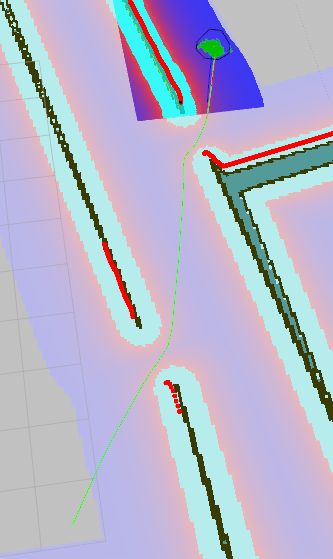
\includegraphics[width=\linewidth]{NC_hi.png}
%	\caption{\mintinline{bash}{neutral_cost} = 233}
%	\endminipage\hfill
%\end{figure}

\begin{figure}[!htb]
	\begin{minipage}[t]{0.33\linewidth}
		\centering 
		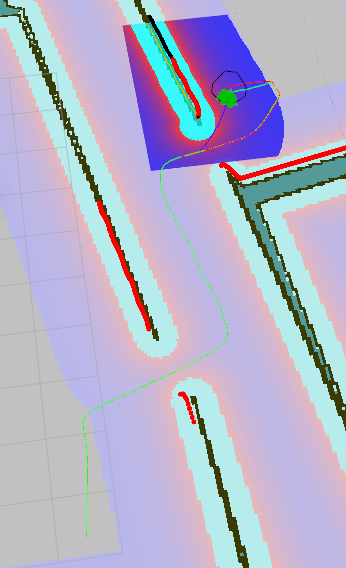
\includegraphics[width=\linewidth]{NC_lo.png}
		\caption{\mintinline{bash}{neutral_cost} = 1}
		%\label{fig:side:a} 
	\end{minipage}\hfill
	\begin{minipage}[t]{0.33\linewidth} 
		\centering 
		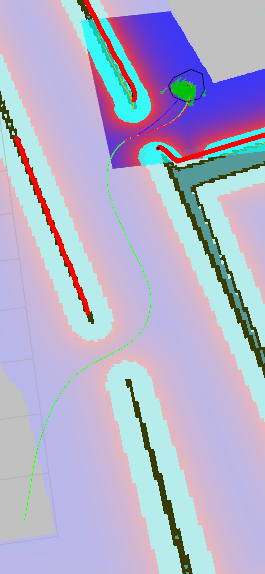
\includegraphics[width=\linewidth]{NC_mid.png}
		\caption{\mintinline{bash}{neutral_cost} = 66}
		%		\label{fig:side:b} 
	\end{minipage}\hfill 
	\begin{minipage}[t]{0.33\linewidth} % 如果一行放2个图,用0.5,如果3个图,用0.33
		\centering 
		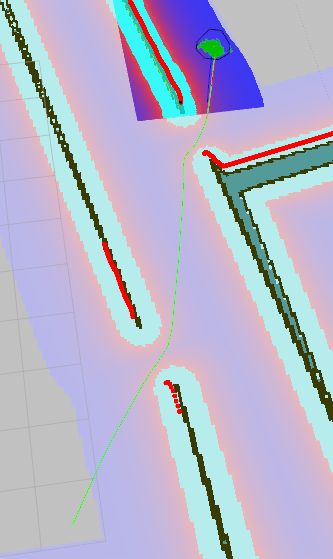
\includegraphics[width=\linewidth]{NC_hi.png}
		\caption{\mintinline{bash}{neutral_cost} = 233}
		%	 	\label{fig:side:a} 
	\end{minipage}% 
\end{figure}

在\mintinline{bash}{navfn} 中,代价值计算方式为:

$$\texttt{cost = COST\_NEUTRAL + COST\_FACTOR * costmap\_cost\_value.}$$

\noindent 传入costmap的代价值的范围为0到255。注解中提到:
\begin{displayquote} 
	\kaishu
	当\mintinline{bash}{COST_NEUTRAL}为50时,\mintinline{bash}{COST_FACTOR}需要设置为大约0.8以确保输入值均匀分布到50到253的输出范围内。
	如果 \mintinline{bash}{COST_FACTOR} 设置为更高的值,则代价值将稳定到障碍物的高度,规划器会不重视狭窄走廊的宽度,不会沿着中心规划路径。
\end{displayquote}

\paragraph[Experiment observations]{实验观察} %
实验也证实了这些解释。将\mintinline{bash}{cost_factor}设置得太低或太高都会降低路径的质量。这些路径并不会穿过每侧障碍物的中间,并具有相对低较的曲率。
极端的\mintinline{bash}{COST_NEUTRAL}值具有类似的效果。
对于\mintinline{bash}{lethal_cost},将其设置为较低的值可能导致无法生成任何路径,即使可行路径仍非常明显。图$5-10$显示了\mintinline{bash}{cost_factor} 和\mintinline{bash}{neutral_cost}在全局规划任务上的效果。其中绿线是\mintinline{bash}{global_planner}规划的全局路径。

经过几次试验后,我们看到,当\mintinline{bash}{cost_factor} = 0.55, \mintinline{bash}{neutral_cost} = 66, 和 \mintinline{bash}{lethal_cost} = 253时,生成的全局路径是我们想要得到的路径。

\section[Local Planner Selection]{局部规划器的选择}

继承自\mintinline{bash}{nav_core::BaseLocalPlanner}接口的局部规划器有\mintinline{bash}{dwa_local_planner} (dwa局部规划器), \mintinline{bash}{eband_local_planner} (eband局部规划器)和 \mintinline{bash}{teb_local_planner} (teb局部规划器)。
它们使用不同的算法生成速度指令。
一般而言,\mintinline{bash}{dwa_local_planner}使得得较多,
我们将对它进行详细讨论。
其它规划器的信息稍后将会提供。

\subsection[DWA Local Planner]{DWA局部规划器}
\subsubsection[DWA algorithm]{DWA算法}

\mintinline{bash}{dwa_local_planner}使用动态窗口(Dynamic Window Approach, DWA)算法。ROS的Wiki页面提供了该算法的实现总结:

\begin{center}
	\setlength{\fboxsep}{1em}
	\fbox{\begin{minipage}{33 em}
			\begin{enumerate}
				\kaishu
				\item 在机器人的控制空间\textit{(dx,dy,dtheta)}进行离散采样。
				\item 对于每个采样速度,从机器人的当前状态执行正向模拟,预测使用该采样速度在某个(短)时间段内会发生什么情况。
				\item %利用包含有以下因子的度量来评估(计分)每个由前向模拟产生的轨迹:接近障碍物程序,接近目标程序,与全局路径的接近性
				使用含有以下因素的度量来评估(得分)每个前向模拟产生的轨迹:与障碍物的接近度,与目标点的接近度,全局路径的贴合度,及所使用的速度。 丢弃不合格的轨迹(与障碍物发生碰撞的轨迹)。
				\item 选择得分最高的轨迹并将相关的速度指令发送到移动基座。
				\item 清零(Rinse)并重复该过程。
			\end{enumerate}
	\end{minipage}}
\end{center}

DWA由\cite{fox1997dynamic}提出。根据论文描述,DWA的目标是产生一对$(v,\omega)$对,表示最适合机器人局部条件的圆形轨迹。DWA通过在下一个时间间隔中搜索速度空间来达到此目标。该空间中的速度被限制为允许的,这意味着机器人必须能够在到达由这些允许的速度决定的圆形轨迹上的最近障碍物之前停止。此外,DWA将仅考虑动态窗口内的速度,动态窗口被定义为在给定当前平移和旋转速度和加速度的情况下在下一时间间隔内可到达的速度对的集合。DWA最大化目标函数,其取决于(1)到目标的进展,(2)从障碍物的清除,以及(3)前向速度以产生最佳速度对。

我们看看ROS Wiki上的算法概要。第一步对在位于动态窗口内的速度空间中对速度对$(v_x, v_y, \omega)$进行采样。
第二步基本上是剔除不可用的速度(即消除不好的轨迹)。
第三步是利用目标函数评估得到的速度对,产生\emph{轨迹分数}。
第四步和第五步很容易理解:选择对当前状态最好的速度再重新计算。

DWA规划器依赖于提供障碍信息的代价图。因此,调整局部代价图的参数对于优化DWA局部规划器的行为至关重要。下面,
我们通过前向模拟、轨迹评分和代价图等看看相关的参数。


\subsubsection[DWA Local Planner : Forward Simulation]{DWA局部规划器:前向模拟}
前向模拟是DWA算法的第二步。
在该步中,局部规划器将在机器人的控制空间中采样速度,检查由这些速度样本表示的圆形轨迹,最后消除不良速度(轨迹与障碍物相交的速度)。
在设置的时间间隔内,每个由参数 \mintinline{bash}{sim_time}(单位为$s$)控制的速度被模拟为应用到真实机器人上。
我们可以认为\mintinline{bash}{sim_time}是机器人在给定的采样速度下允许运行的时间。

通过实验,我们观察到仿真时间\mintinline{bash}{sim_time}越长,计算负荷越大。此外,当仿真时间\mintinline{bash}{sim_time}变大后,局部路径规划器产生的路径也会相应变长,这种现象是在合理范围内的。
这里有一些关于如何调整仿真时间参数\mintinline{bash}{sim_time}的建议。

\paragraph[How to tune \texttt{sim\_time}]{如何调整\texttt{sim\_time}}

如果将仿真时间\mintinline{bash}{sim_time}的值设置为非常低(例如$\leq 2.0$)将导致性能下降,
尤其是当机器人需要通过狭窄的门口、或家具之间的间隙时。
这是因为没有足够多的时间进行计算以获得最佳轨迹以便通过狭窄的通道。
另一方面,由于使用了DWA规划器,所有的轨迹都是简单的圆弧,如果将仿真时间\mintinline{bash}{sim_time}设置的非常高($\geq$5.0),将得到一条很长的缺乏灵活性能的曲线。该问题并不是不可避免的,因为规划器在每个时间间隔后都会主动进行重规划(由参数\mintinline{bash}{controller_frequency}(单位为$Hz$)控制),它可以对结果进行一次较小的调整。
对于性能较高的计算机,4.0秒的计算时间足矣。


\begin{figure}[!htb]
	\minipage{0.49\textwidth}
	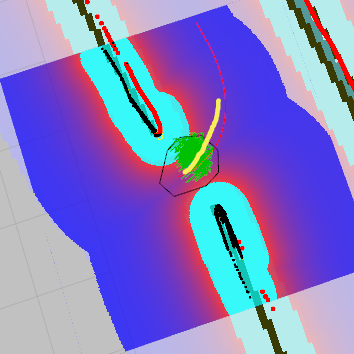
\includegraphics[width=\linewidth]{simtime15.png}
	\caption{\mintinline{bash}{sim_time} = 1.5}
	\endminipage\hfill
	\minipage{0.49\textwidth}
	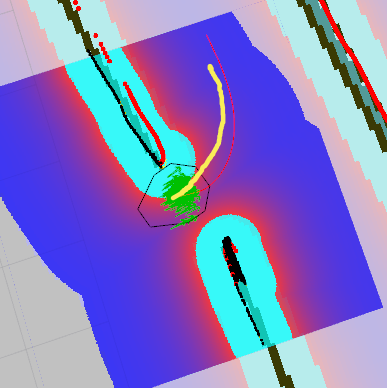
\includegraphics[width=\linewidth]{simtime4.png}
	\caption{\mintinline{bash}{sim_time} = 4.0}
	\endminipage\hfill
\end{figure}

除了仿真时间,还有几个参数值得注意。

\textbf{速度采样}:在其它几个参数中,
\mintinline{bash}{vx_sample}和\mintinline{bash}{vy_sample}分别决定在x和y方向上进行速度采样时平移部分的量。
\mintinline{bash}{vth_sample}控制速度采样中旋转部分的量。
速度采样的数量取决于你的设备的计算能力。
多数情况下,我们倾向于设置\mintinline{bash}{vth_samples}的值大于平移部分的值,原因在于通常情况下旋转要比直线前进更为复杂。
如果将\mintinline{bash}{max_vel_y}设置为零,因为没有可用信息所以没必要在y方向提取速度样本。
我们设置\mintinline{bash}{vx_sample} = 20, \mintinline{bash}{vth_samples} = 40。

\textbf{仿真粒度}:\mintinline{bash}{sim_granularity}意为在轨迹上的采样点之间的步长。
该参数含义为需要多频繁的检查轨迹上的点(检测它们是否与障碍物相交)。
较低的值意味着高频率,当然需要更多的计算性能。
对于turtlebot这类机器人来说,默认值0.025足够胜任。

\subsubsection[DWA Local Planner: Trajactory Scoring]{DWA局部规划器:轨迹得分}

如上所述,DWA规划器通过最大化目标函数来获得最佳速度对。
在DWA的论文中,目标函数的值依赖于三部分:到目标点的过程、清除障碍物和前进速度。在ROS中,目标函数的计算公式如下:

\begin{eqnarray*}\footnotesize
	cost &=& \texttt{path\_distance\_bias} * (\text{distance($m$) to path from the endpoint of the trajectory})\\
	&+& \texttt{goal\_distance\_bias} * (\text{distance($m$) to local goal from the endpoint of the trajectory})\\
	&+& \texttt{occdist\_scale} * (\text{maximum obstacle cost along the trajectory in obstacle cost (0-254)})
\end{eqnarray*}

目标函数的意义在于获得最小的行走代价。
\mintinline{bash}{path_distance_bias}为局部规划器以多大权重与全局路径保持一致\cite{furrer2016robot}。
较大值将使局部规划器倾向于跟踪全局路径。

\mintinline{bash}{goal_distance_bias}衡量机器人无论走哪条路径应该以多大权重尝试到达目标点。
实验显示增加\mintinline{bash}{goal_distance_bias}的值会使机器人与全局路径的一致性保持度偏低。

\mintinline{bash}{occdist_scale}是权衡机器人以多大的权重躲避障碍物。该值过大会导致机器人陷入困境。

在SCITOS G5上,我们设置 \mintinline{bash}{path_distance_bias}为32,\mintinline{bash}{goal_distance_bias}为20,\mintinline{bash}{occdist_scale} 为0.02,仿真结果良好。

\subsubsection[DWA Local Planner: Other Parameters]{DWA局部规划器:其他参数}%{DWA Local Planner : Other Parameters}

主要目标距离公差(Goal distance tolerance):这些参数很直观,以下为它们在ROS Wiki上的描述\footnote{译者注:适当更改这些参数可解决机器人原地转圈的问题,例如\url{https://blog.csdn.net/Enterenvy/article/details/90699274}。}:

\begin{itemize}
	\item \mintinline{bash}{yaw_goal_tolerance} (double, 默认值: 0.05,单位:弧度)
	%The tolerance in radians for the controller in yaw/rotation when achieving its goal.
	到达目标点时,偏航/旋转中控制器的弧度公差(tolerance)。
	
	\item \mintinline{bash}{xy_goal_tolerance} (double, 默认值: 0.10,单位:米)
	%The tolerance in meters for the controller in the x \& y distance when achieving a goal.
	到达目标点时,控制器在x \& y方向的距离公差,单位为米。
	
	\item \mintinline{bash}{latch_xy_goal_tolerance} (bool, 默认值: false) 
	%If goal tolerance is latched, if the robot ever reaches the goal xy location it will simply rotate in place, even if it ends up outside the goal tolerance while it is doing so.
	目标公差被锁定情况下,机器人到达目标的xy位置时会简单旋转到位;
	如果机器人在目标公差(goal tolerance)范围之外进入结束状态时,也会简单旋转到位。
	
\end{itemize}

\textbf{振荡复位}(Oscilation reset):
在诸如通过门口情况下,机器人可能会来回振荡,因为其局部规划器正在产生通过两个相反方向的路径。如果机器人保持振荡,导航功能包将让机器人尝试恢复行为。

\begin{itemize}
	\item \mintinline{bash}{oscillation_reset_dist} (double, 默认值: 0.05, 单位:米) 
	%How far the robot must travel in meters before oscillation flags are reset.
	机器人必须运动多少米远后才能复位震荡标记。即:来回运动在多大距离以上不会被认为是振荡。
\end{itemize}



\section[Costmap Parameters]{代价地图参数}
如上所述,代价地图参数对于本地规划器(不仅仅是DWA)是至关重要的。在ROS中,代价地图由静态地图层、障碍物图层和膨胀层组成。
静态地图层直接给导航堆栈提供静态SLAM地图解释。
障碍物图层包含2D障碍物和3D障碍物(体素层)。
膨胀层是将障碍物膨胀来计算每个2D代价地图单元的代价。

如上所述,调整\textit{costmap}代价地图参数对于局部规划器(不仅仅是DWA)的成功至关重要。 
在ROS中,costmap由静态地图层(static map layer),障碍地图层(obstacle map layer)和膨胀层(inflation layer)组成。 
静态地图层对提供给导航功能包的静态SLAM地图直接进行解释。 
障碍层包括有2D的障碍物和3D的障碍物(体素层)。 
膨胀层将障碍物进行膨胀以计算每个2D代价单元(cell)的通行代价。

此外,还存在全局代价地图(\textit{global costmap}),和局部代价地图(\textit{local costmap})。
全局代价地图通过膨胀导航功能包的地图上已存在的障碍物产生。
局部代价地图通过将机器人传感器检测到的障碍物进行膨胀产生的。

\begin{figure}[!h]
	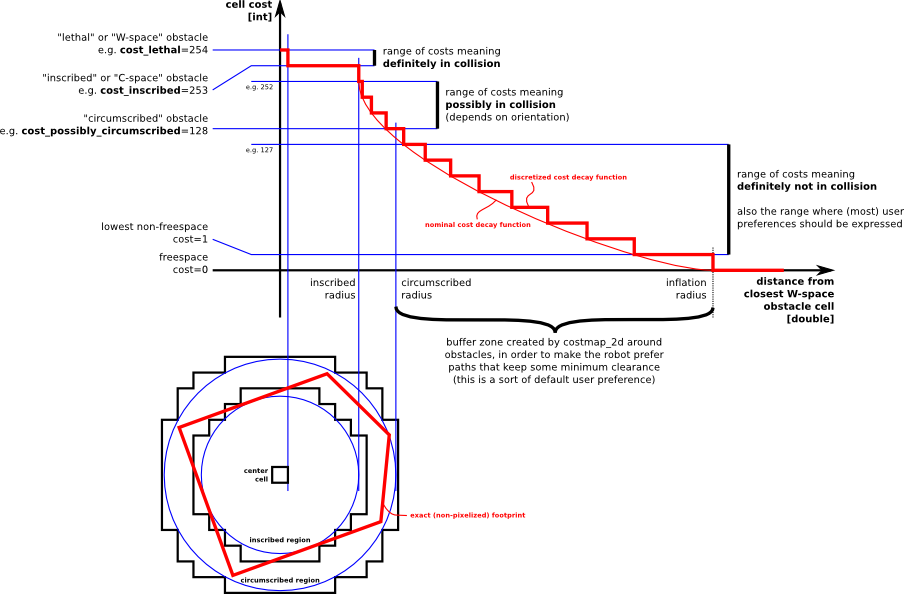
\includegraphics[width=\linewidth]{costmapspec.png}
	\caption{膨胀衰减}
\end{figure}

\noindent 此外还有很多重要的参数应尽可能设置好。

\subsection[footprint]{足迹}%{footprint} 

足迹(footprint)是机器人移动本体的轮廓。
在ROS中,footprint由二维数组表示 $[x_0, y_0], [x_1,y_1], [x_2,y_2], ...]$,无需重复第一个坐标。
footprint用于计算内切圆和外接圆的半径,以确定适合该机器人的方式对障碍物进行膨胀。
为安全起见,我们通常将footprint设置为略大于机器人的真实轮廓。

要确定机器人的footprint,最直接的方法是参考机器人的图纸。 
此外,您可以手工拍摄其基座俯视图。 然后使用CAD软件(例如Solidworks)适当缩放图像,并将鼠标移动到基座轮廓周围并读取其坐标。 
坐标原点应为机器人的中心。 
或者,您可以将机器人移动到一张大纸上,然后绘制基座的轮廓。 然后选择一些顶点并使用标尺来确定它们的坐标。

\subsection[inflation]{膨胀}%{inflation} 
膨胀层(Inflation layer)由代价值位于0到255的单元(cell)组成。每个单元可能会被占据(occupied)、无障碍或未知三种情况。
图13的图表\footnote{图表来自\url{http://wiki.ros.org/costmap_2d}}说明了如何计算膨胀衰减曲线的过程。

\mintinline{bash}{inflation_radius}\mintinline{bash}{cost_scaling_factor}是决定膨胀的主要参数。
\mintinline{bash}{inflation_radius}控制零代价点距离障碍物有多远。
\mintinline{bash}{cost_scaling_factor}与单元(cell)的代价值成反比,设置高值将使衰减曲线更为陡峭。

Pronobis博士认为,最佳代价图的衰减曲线应为斜率相对较低的曲线,这样可使得最佳路径尽可能远离每侧的障碍物。
优点是机器人更趋向于在障碍物中间移动。
如图8和图9所示,在具有相同的起点和目标点情况下,当代价图的曲线非常陡峭时,机器人往往会靠近障碍物。
在图14中,膨胀半径\mintinline{bash}{inflation_radius} = 0.55,代价比例因子\mintinline{bash}{cost_scaling_factor} = 5.0;在图15中,膨胀半径\mintinline{bash}{inflation_radius} = 1.75,代价比例因子\mintinline{bash}{cost_scaling_factor} = 2.58。

%\begin{figure}[!htb]
%	\minipage{0.49\textwidth}
%	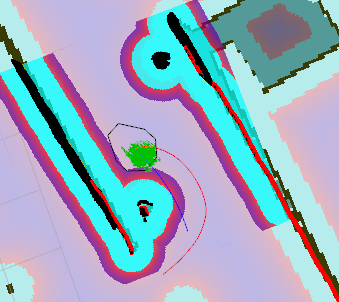
\includegraphics[width=\linewidth]{notgoodinflation.png}
%	\caption{steep inflation curve}
%	\endminipage\hfill
%	\minipage{0.49\textwidth}
%	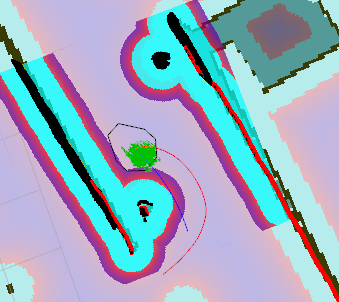
\includegraphics[width=\linewidth]{notgoodinflation.png}
%	\caption{gentle inflation curve}
%	\endminipage\hfill
%\end{figure}

\begin{figure}[!htb]
	\begin{minipage}[t]{0.49\linewidth}
		\centering 
		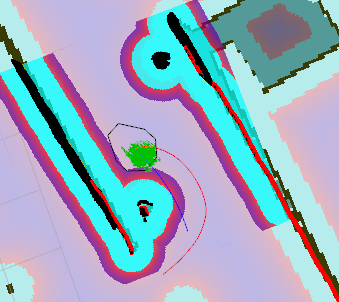
\includegraphics[width=0.98\linewidth]{notgoodinflation.png} 
		\caption{陡峭的膨胀曲线} 
		\label{fig:side:a} 
	\end{minipage}% 
	\begin{minipage}[t]{0.49\linewidth} 
		\centering 
		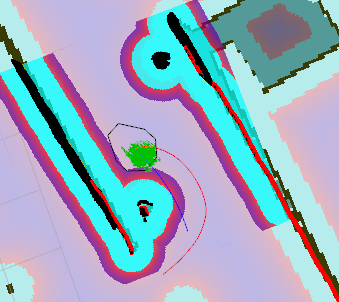
\includegraphics[width=0.98\linewidth]{notgoodinflation.png} 
		\caption{温和的膨胀曲线} 
		\label{fig:side:b} 
	\end{minipage} 
\end{figure}

根据衰变曲线图,我们需设定这两个参数值,以使得膨胀半径几乎覆盖走廊,并且代价值的衰减速度相对中等,这意味着要降低代价的比例因子\mintinline{bash}{cost_scaling_factor}的值。

\subsection[costmap resolution]{代价地图的分辨率}%{costmap resolution} 
可以在局部代价图和全局代价图单独设置此参数。它们影响着计算设备的计算负荷和规划器的路径规划能力。
对于低分辨率($>=0.05$),在狭窄的通道中,障碍物区域可能会重叠,导致局部规划器无法找到可通行路径。

对于全局代价图的分辨率,只要其与导航功能包的地图的分辨率保持相同即可。
如果有足够的计算能力,可以查看激光扫描仪的分辨率,因为当使用gmapping建图时,如果激光扫描仪的分辨率低于所需的地图分辨率,则会有很多小的“未知点”,因为激光扫描仪无法覆盖该区域,如图10所示。


\begin{figure}[!h]
	\begin{center}
		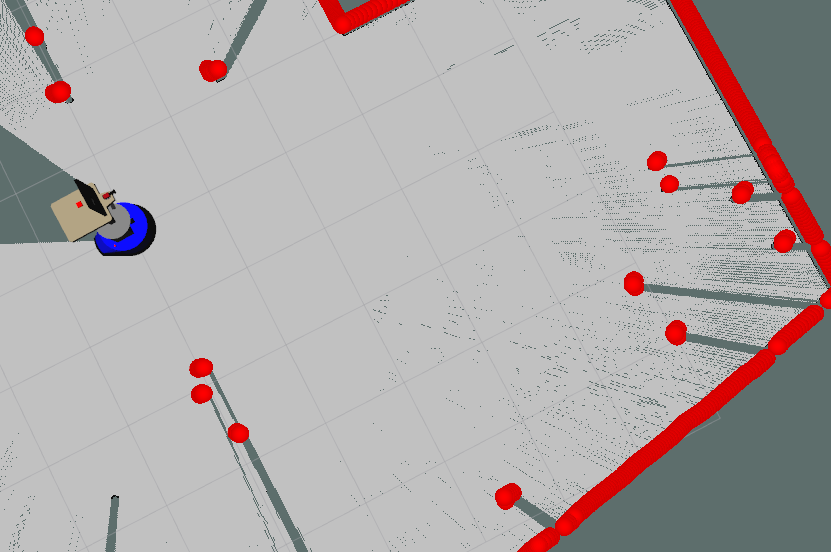
\includegraphics[width=22em]{resolutionholes.png}
		\caption{gmapping分辨率= 0.01。 注意图像右侧的未知点}
		%{gmapping resolution = 0.01. Notice the unknown dots on the right side of the image}
	\end{center}
\end{figure}

例如,Hokuyo URG-04LX-UG01激光扫描仪的分辨率是0.01mm\footnote{数据来源: \url{https://www.hokuyo-aut.jp/02sensor/07scanner/download/pdf/URG-04LX_UG01_spec_en.pdf}},因此建立扫描分辨率为$\leq 0.01$的地图需要多旋转机器人几次才能清除未知的点。
可以发现,0.02的分辨率就够用了。

\subsection[obstacle layer and voxel layer]{障碍物层和体素层}
这两个图层负责在代价图上标注障碍物。它们可以被称为障碍层(\textit{obstacle layer})。根据ROS wiki的介绍,障碍层在两个维度上进行跟踪,而体素层在三个维度上进行跟踪。障碍物是根据机器人传感器的数据进行标记(检测)或清除(删除)建立的,
同时为代价图提供了订阅的主题(topics)。

在ROS的实现代码中,体素层继承自障碍物层,两者皆为通过解释激光扫描(laser scans)或使用\mintinline{bash}{PointCloud}和\mintinline{bash}{PointCloud2}类型的消息发送数据获取障碍物的信息。 此外,体素层需要深度传感器,如Microsoft Kinect或ASUS Xtion。 3D障碍物最终会被膨胀为二维代价图。

\textbf{体素层如何工作}:
体素是空间中具有一定相对位置的3D立方体(想象为3D像素)。它用于与其附近的数据或属性进行关联。例如,它的位置是否为一个障碍。
与体素与深度相机相关的3D重建已经有很多研究了。
已经存在很多通过深度相机获取体素进行在线3D重建的研究了。这是其中的一部分。

\begin{itemize}
	\item \href{http://delivery.acm.org/10.1145/2050000/2047270/p559-izadi.pdf?ip=128.208.7.188&id=2047270&acc=ACTIVE\%20SERVICE&key=B63ACEF81C6334F5\%2EF43F328D6C8418D0\%2E4D4702B0C3E38B35\%2E4D4702B0C3E38B35&CFID=830915711&CFTOKEN=23054788&__acm__=1472349664_9fd28ae246d72a507f6a93c5ac84a516}{KinectFusion: Real-time 3D Reconstruction and Interaction Using a Moving Depth Camera} 
	\item \href{https://people.mpi-inf.mpg.de/~mzollhoef/Papers/SGASIA2013_VH/paper.pdf}{Real-time 3D Reconstruction at Scale using Voxel Hashing}
	% \item \href{https://www.ri.cmu.edu/pub_files/2014/6/VoxelCarving.pdf}{Object Modeling and Recognition from Sparse, Noisy Data via Voxel Depth Carving}
\end{itemize}

体素网格\mintinline{bash}{voxel_grid}是一个ROS包,它提供了一个高效的三维体素网格数据结构的实现,该存储了体素的三种状态:标记状态(marked)、自由状态(free)、未知状态(unknown)。\mintinline{bash}{voxel_grid}占据了代价地图区域内的体积。
在每次更新体素边界期间,体素层根据传感器的数据来标记或移除体素网格中的一些体素。
它还执行光线跟踪(ray tracing)作用,该内容将在接下来进行讨论。
请注意,体素层在更新时,不会重新创建体素网格;仅在更改局部代价图的尺寸大小时体素层才进行更新。

为什么要在障碍物层或体素层进行光线跟踪?
光线跟踪以渲染逼真的3D图形而闻名,因此读者可能会对为什么将它用于处理障碍物这个问题而倍感困惑。
一个重要的原因是可以通过机器人的传感器检测不同类型的障碍物。
请观察图17。
理论上,我们还可以知道障碍物是刚性的还是柔性的(例如草)\footnote{出处为:\textit{Using Robots in Hazardous Environments}, Boudoin, Habib, pp.370。}。

\begin{figure}[!h]
	\begin{center}
		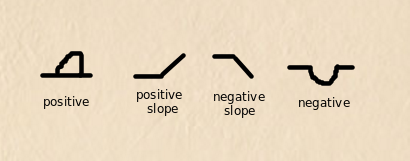
\includegraphics[width=23em]{ObstacleTypes.png}
		\caption{通过光线跟踪,激光扫描仪能够识别不同类型的障碍物。}
		%{With ray tracing, laser scanners is able to recognize different types of obstacles.}
	\end{center}
\end{figure}

一个关于体素光线跟踪对比多声源追踪的好博客:
\url{http://raytracey.blogspot.com/2008/08/voxel-ray-tracing-vs-polygon-ray.html} 

通过以上的解释,我们来研究一下障碍物层的一些参数\footnote{个别解释直接拷贝自ROS Wiki对costmap2d的介绍}。这些参数属于全局滤波参数,对所有的传感器都是适用的。

\begin{itemize}
	\item \mintinline{bash}{max_obstacle_height}: 
	%	The maximum height of any obstacle to be inserted into the costmap in meters. This parameter should be set to be slightly higher than the height of your robot. For voxel layer, this is basically the height of the voxel grid.
	以米为单位插入代价图中的障碍物的最大高度。该参数应设置为略高于机器人的最大高度。对于体素层,这本质含义是指体素网格的高度。
	
	\item \mintinline{bash}{obstacle_range}: 
	%	The default maximum distance from the robot at which an obstacle will be inserted into the cost map in meters. This can be over-ridden on a per-sensor basis.
	插入代价地图的障碍物应距离机器人的最大默认距离,以米为单位。它可以在每个传感器的基础上进行覆盖操作。
	
	\item \mintinline{bash}{raytrace_range}: 
	%The default range in meters at which to raytrace out obstacles from the map using sensor data. This can be over-ridden on a per-sensor basis.
	%用于使用传感器数据在地图中扫描出障碍物,以米为单位,可以在每个传感器的基础上进行覆盖
	使用传感器数据从地图中扫描出障碍物的最大距离范围(以米为单位)。 同样,该值可以在每个传感器的基础上进行覆盖。
	
\end{itemize}

%These parameters are only used for the voxel layer (VoxelCostmapPlugin).
下面的这些参数仅适用于体素层(VoxelCostmapPlugin)
\begin{itemize}
	\item \mintinline{bash}{origin_z}: 
	%The z origin of the map in meters.
	地图的Z轴原点,以米为单位
	\item \mintinline{bash}{z_resolution}: 
	%	The z resolution of the map in meters/cell.
	地图的Z轴分辨率,以\emph{米/单元格}(meters/cell)为单位。
	
	\item \mintinline{bash}{z_voxels}: 
	%	The number of voxels to in each vertical column, the height of the grid is z_resolution * z_voxels.
	每个垂直列中的体素数目,网格的高度为\mintinline{bash}{z_resolution * z_voxels}。
	
	\item \mintinline{bash}{unknown_threshold}: 
%	The number of unknown cells allowed in a column considered to be "known"
	当整列的voxel是“已知”(``known'')的时候,含有的未知cell(“unknown”)的最大数量。
	
	\item \mintinline{bash}{mark_threshold}: 
	%	The maximum number of marked cells allowed in a column considered to be "free".
	%	在被认为是“自由”的列中允许的标记单元的最大数量
	整列voxel认为是“自由”("free")的时候,含有的已标记的cell(“marked”)的最大数目。
	
\end{itemize}

\paragraph[Experiment observations]{实验观察情况}%{Experiment observations} 

实验进一步阐明了体素层参数的影响。我们使用ASUS Xtion Pro作为深度传感器。 我们发现Xtion的位置很重要,它决定了“盲区”的范围,即深度传感器看不到任何东西的区域。

此外,当障碍物出现在Xtion的范围内时,表示障碍物的体素才会进行更新(标记或清除)。
否则,一些体素的信息仍保持不变,在代价地图中的膨胀信息也会保留。

另外,Z轴分辨率 \mintinline{bash}{z_resolution} 灰顶Z轴体素的密度。如果值很高,体素层会很密集。
如果值太低(例如0.01),所有的体素将被放在一起,将不会获得有效的代价图信息。如果将Z轴分辨率设置为较高的值,意图是更好地获得障碍物,因此需要增加Z轴体素数(该参数控制每个垂直列中的体素数)。如果列中的体素数太多但分辨率不够也是没用的,因为每个垂直列的高度都有限制。图18-20显示了不同体素参数设置之间的比较。

另外,Z轴的分辨率参数\mintinline{bash}{z_resolution}控制体素在$ z $-轴上的密度。 如果值很高,则体素层会更密集。 
如果该值太低(例如0.01),则所有体素将被放在一起,因此您将无法获得有用的代价图信息。 
如果将\mintinline{bash}{z_resolution}设置为更高的值,您的愿望应该是更好地获得障碍,因此您需要增加\mintinline{bash}{z_voxels}参数来控制每个垂直列中的体素数。 如果列中的体素太多但分辨率不够会导致设置不起作用,因为每个垂直列的高度都有限制。 
图18-20展示了设置不同的体素层参数进行比较的效果。

\begin{figure}[!h]
\end{figure}

\begin{figure}[!h]
	\minipage{0.32\textwidth}
	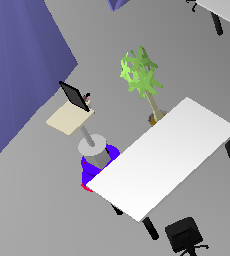
\includegraphics[width=\linewidth]{voxellayerscene.png}
	\caption{场景:植物在机器人前面}
	\endminipage\hfill
	\minipage{0.32\textwidth}
	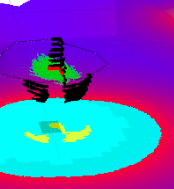
\includegraphics[width=\linewidth]{voxellayerparam1.png}
	\caption{较高的\mintinline{bash}{z_resolution}}
	\endminipage\hfill
	\minipage{0.32\textwidth}
	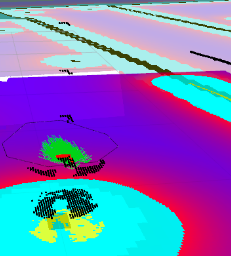
\includegraphics[width=\linewidth]{voxellayerparam2.png}
	\caption{较低的\mintinline{bash}{z_resolution}}
	\endminipage\hfill
\end{figure}

%%%%%%%%%%%%%%%%%%%%%%%%%%%%%%%%

\section[AMCL]{AMCL}

\mintinline{bash}{amcl} 是一个处理机器人定位的ROS包。 它是Adaptive Monte Carlo Localization(自适应蒙特卡罗, AMCL)的缩写,也称为粒子滤波(partical filter)定位器。 这种定位技术的工作原理如下:每个样本都存储一个表示机器人姿态的位置和方向数据。 
粒子在开始状态时都是随机采样的。 
当机器人移动时,粒子将根据其当前状态以及机器人的动作使用递归贝叶斯估计(recursive Bayesian estimation)进行重新采样。

稍后将提供更多关于调整AMCL参数的讨论。请参考ROS维基\url{http://wiki.ros.org/amcl}以了解更多信息。关于原始Monte Carlo Localization (蒙特卡罗,MCL)的算法细节,阅读由Thrun, Burgard, 和 Fox所著的《概率机器人》(《Probabilistic Robotics》第八章\cite{thrun2005probabilistic}。

我们现在总结一些可能影响AMCL定位质量的问题\footnote{于2019年4月8日增加。此指南于2017年5月完成,当时未在本指南中报告该部分内容。}。 我们希望此信息能够使本指南更加完整,并且您觉得有用。

\begin{figure}[!tb]
	\minipage{0.49\textwidth}
	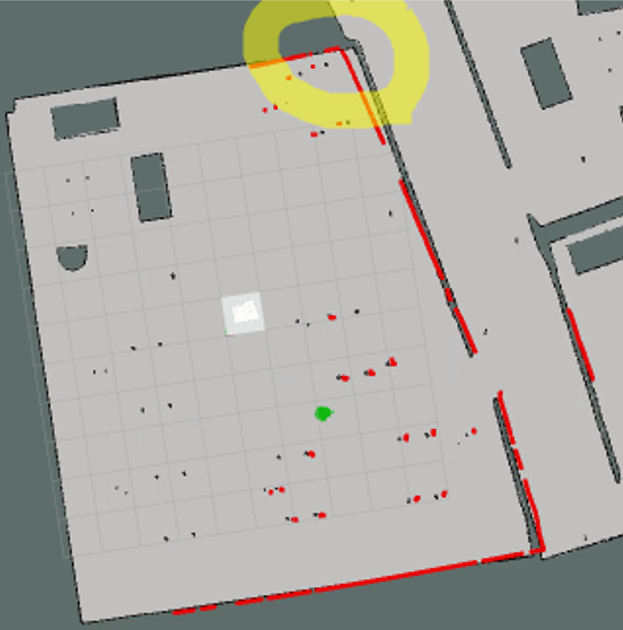
\includegraphics[width=\linewidth]{scanner1.png}
	\caption{当\mintinline{bash}{LaserScan} 字段不正确时}
	%{When \mintinline{bash}{LaserScan} fields are not correct}
	\label{fig:scanner1}
	\endminipage\hfill
	\minipage{0.49\textwidth}
	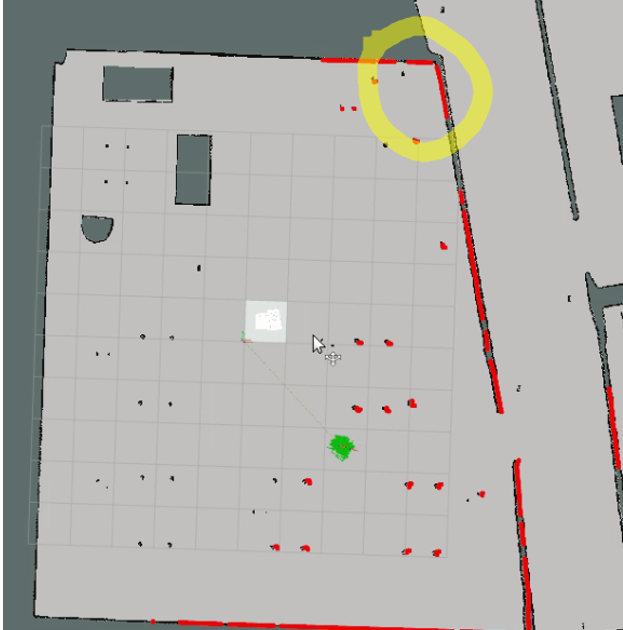
\includegraphics[width=\linewidth]{scanner2.png}
	\caption{当\mintinline{bash}{LaserScan} 字段正确时}
	%{When \mintinline{bash}{LaserScan} fields are correct}
	\label{fig:scanner2}
	\endminipage\hfill
\end{figure}

通过实验,我们观察到三个影响AMCL定位的问题。 正如\cite{thrun2005probabilistic}中所述,MCL维护两个概率模型,
一个\emph{运动模型}(motion)和一个\emph{测量模型}(measurement)。 
在ROS的\mintinline{bash}{amcl}中,运动模型对应于里程计的模型,而测量模型对应于激光扫描的模型。 
通过这种理解,我们分别描述了三个问题归结如下。

\subsection[Header in \texttt{LaserScan} messages]{ \texttt{LaserScan}的头部结构问题}%{Header in \mintinline{bash}{LaserScan} messages}

发布到\mintinline{bash}{scan}主题的消息类型为\mintinline{bash}{sensor_msgs/LaserScan}\footnote{请参阅:\url{http://docs.ros.org/melodic/api/sensor_msgs/html/msg/LaserScan.html}}。此消息包含一个header部分,其字段取决于您所使用的具体的激光扫描仪。这些字段包括(以下内容摘自该消息的说明文档)

\begin{itemize}
	\item \mintinline{bash}{angle_min} (float32) scan的开始角度 [弧度] % [单位:rad (弧度)] %start angle of the scan [rad]
	\item \mintinline{bash}{angle_max} (float32) scan的结束角度 [弧度] %[单位:rad (弧度)]  %end angle of the scan 
	\item \mintinline{bash}{angle_increment} (float32) 测量的角度间的距离 [弧度] % start angle of the scan [rad]
	\item \mintinline{bash}{time_increment} (float32) 测量间的时间 [秒] -- 如果扫描仪在移动,这将用于插入3D点的位置 %time between measurements [seconds] - if your scanner is moving, this will be used in interpolating position of 3d points
	\item \mintinline{bash}{scan_time} (float32) 扫描间的时间 [秒] %time between scans [seconds]
	\item \mintinline{bash}{range_min} (float32) 最小的测量距离 [米]%minimum range value [m]
	\item \mintinline{bash}{range_max} (float32) 最大的测量距离 [米] %maximum range value [m]
	
	\item \mintinline{bash}{ranges} (float32 [])  测量的距离数据 [米] (注意: 值 < range\_min 或 > range\_max 应当被丢弃)
	\item \mintinline{bash}{intensities} (float32 []) 强度数据 [与设备相关的单位]
\end{itemize}

我们在实验中观察到,如果没有为机器人身上的激光扫描仪正确设置这些参数的值,将影响定位的质量
(参见图\ref{fig:scanner1}和图\ref{fig:scanner2}。我们使用了两个激光扫描仪,SICK LMS 200和SICK LMS 291。我们提供它们的参数如下\footnote{对LMS 200,感谢该\emph{github}的问题(\url{https://github.com/smichaud/lidar-snowfall/issues/1})}。

\noindent SICK LMS 200:
%\lstset{language=json}
\begin{minted}[frame={leftline},]{xml}
{   
"range_min": 0.0,
"range_max": 81.0,
"angle_min": -1.57079637051,
"angle_max": 1.57079637051,
"angle_increment": 0.0174532923847,
"time_increment": 3.70370362361e-05,
"scan_time": 0.0133333336562
}
\end{minted}

\noindent SICK LMS 291:
%\lstset{language=json}
\begin{minted}[frame={leftline},]{xml}
{   
"range_min": 0.0,
"range_max": 81.0,
"angle_min": -1.57079637051,
"angle_max": 1.57079637051,
"angle_increment": 0.00872664619235,
"time_increment": 7.40740724722e-05,
"scan_time": 0.0133333336562
}
\end{minted}

\subsection[Parameters for measurement and motion models]{测量和运动模型的参数问题}

\mintinline{bash}{amcl}包中列出了有关调整激光扫描仪模型(测量)和里程计模型(运动)的参数。
有关完整列表及其定义,请参阅\mintinline{bash}{amcl}包页面。
对这参数的详细讨论需要理解论文\cite{thrun2005probabilistic}的MCL算法,我们在此省略该部分内容。
我们提供了一个\emph{示例}展示如何调整这些参数,并定性描述它们的结果。
实际参数应根据所使用的激光扫描仪和机器人作调整。

对于\textbf{激光扫描模型},默认的参数为:

%\lstset{language=bash}
\begin{minted}[frame={leftline},]{xml}
{
"laser_z_hit": 0.5,
"laser_sigma_hit": 0.2,
"laser_z_rand" :0.5,
"laser_likelihood_max_dist": 2.0
}
\end{minted}

为了改善机器人的定位精度,我们增加了\mintinline{bash}{laser_z_hit}和\mintinline{bash}{laser_sigma_hit}参数来引入更多噪音测量。最后的参数为:

%\lstset{language=json}
\begin{minted}[frame={leftline},]{xml}
{
"laser_z_hit": 0.9,
"laser_sigma_hit": 0.1,
"laser_z_rand" :0.5,
"laser_likelihood_max_dist": 4.0
}
\end{minted}

机器人的行为如图〜\ref{fig:param1}和\ref{fig:param2}所示。显然,在我们的案例中,在测量模型中增加噪声测量有助于定位。

\begin{figure}[!tb]
	\minipage{0.49\textwidth}
	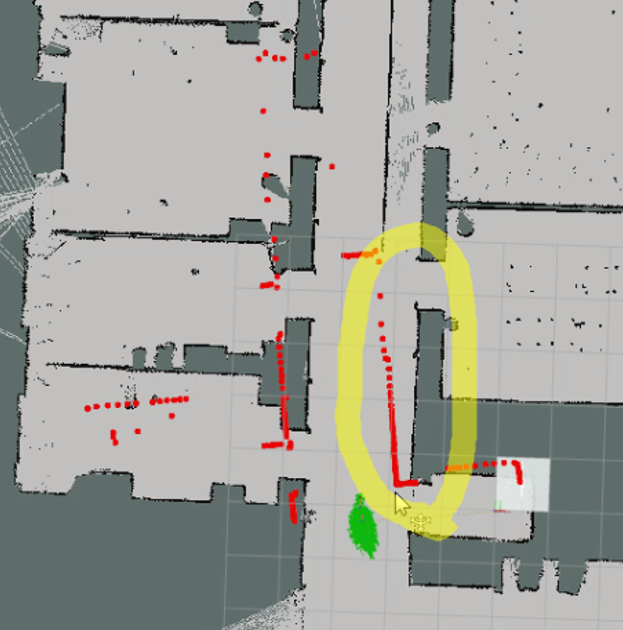
\includegraphics[width=\linewidth]{param1.png}
	\caption{默认测量模型参数}%{Default measurement model parameters}
	\label{fig:param1}
	\endminipage\hfill
	\minipage{0.49\textwidth}
	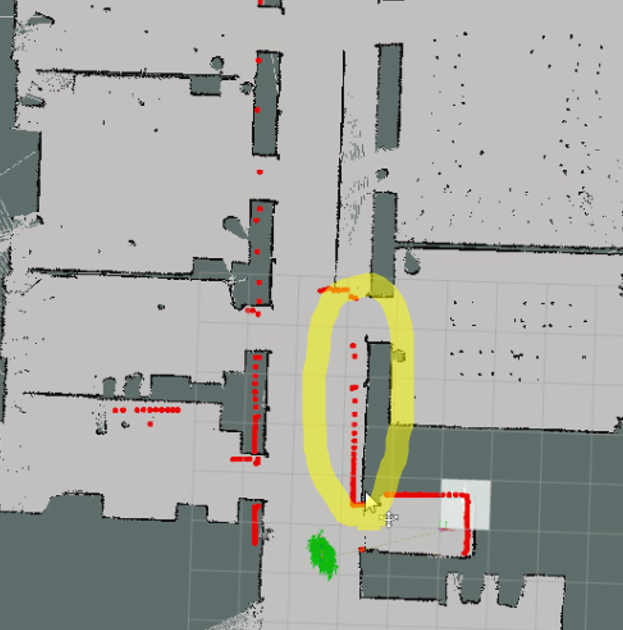
\includegraphics[width=\linewidth]{param2.png}
	\caption{调整测量模型参数后(增加噪声)}%{After tuning measurement model parameters (increase noise)}
	\label{fig:param2}
	\endminipage\hfill
\end{figure}

对于\textbf{里程计模型},我们发现我们的里程计非常稳定。因此,我们调整了参数,便于算法假设里程计中的噪音很低:

%\lstset{language=json}
\begin{minted}[frame={leftline},]{xml}
{   
"kld_err": 0.01,
"kld_z": 0.99,
"odom_alpha1": 0.005,
"odom_alpha2": 0.005,
"odom_alpha3": 0.005,
"odom_alpha4": 0.005
}
\end{minted}

为验证上述参数对运动模型是否有效,我们还尝试了一组受噪声污染的里程模型的建议参数:
%\lstset{language=json}
\begin{minted}[frame={leftline},]{xml}
{
"kld_err": 0.10,
"kld_z": 0.5',                                                                            
"odom_alpha1": 0.008,                                                                     
"odom_alpha2": 0.040,                                                                     
"odom_alpha3": 0.004,                                                                     
"odom_alpha4": 0.025                                                                      
} 
\end{minted}

我们观察到,当里程模型噪声较小时,粒子会更加收缩;否则,粒子会更加分散。

\subsection[Translation of the laser scanner]{激光扫描仪的平移问题}

ROS中有个\mintinline{bash}{tf}变换可以将坐标系从\mintinline{bash}{laser_link}转换为\mintinline{bash}{base_footprint}或\mintinline{bash}{base_link},表示激光扫描仪相对于机器人基座的姿态。如果此变换不正确,则很可能导致机器人的定位行为难以理解。
在那种情况下,我们观察到激光传感器扫描环境中的墙壁时其读数有一定的漂移,并且定位产生剧烈变化。
这种检验方式足够简单,用以确保\mintinline{bash}{tf}变换无误;
通常在机器人的\mintinline{bash}{urdf}和\mintinline{bash}{srdf}规范中有相应的处理方式。
但是,如果您使用的是\mintinline{bash}{rosbag}文件,则必须自行发布\mintinline{bash}{tf}转换。

%%%%%%%%%%%%%%%%%%%%%%%%%%%%%%%%
\section[Recovery Behaviors]{恢复行为}%{Recovery Behaviors}

机器人导航过程中比较头疼的一个问题是机器人可能会被卡住。 幸运的是,导航功能包内置了恢复行为。 
即便如此,有时机器人会耗尽所有可用的恢复行为后保持静止。因此,我们需要一个更强大的解决方案。

\textbf{恢复行为的种类}:ROS导航功能包有两种恢复行为。它们是\mintinline{bash}{clear_costmap_recovery}和\mintinline{bash}{rotate_recovery}。
清除代价地图恢复本质上是将局部代价地图恢复为与全局代价地图等价的状态。
旋转恢复是通过旋转360°来恢复。

\textbf{解救机器人}:有时由于旋转故障,旋转恢复无法获得执行。此时,机器人可能会选择放弃,因为它已经尝试了所有的恢复行为--清除代价地图和旋转恢复。
我们观察到,在大多数试验中,当机器人选择放弃行为时,实际上仍有很多方法可以解救机器人。
为了避免放弃,我们使用SMACH来连续尝试不同的恢复行为,通过其他额外的行为,例如设置非常接近机器人的临时目标,并返回到以前访问过的姿态(即退出)。这些方法可以显著提高机器人的耐久性,并且从以前观察到的无望空间中解救出来\footnote{这是我在开展移动机器人导航方面的工作时的一个演示视频: \url{https://youtu.be/1-7GNtR6gVk}}。

\begin{figure}[!h]
	\begin{center}
		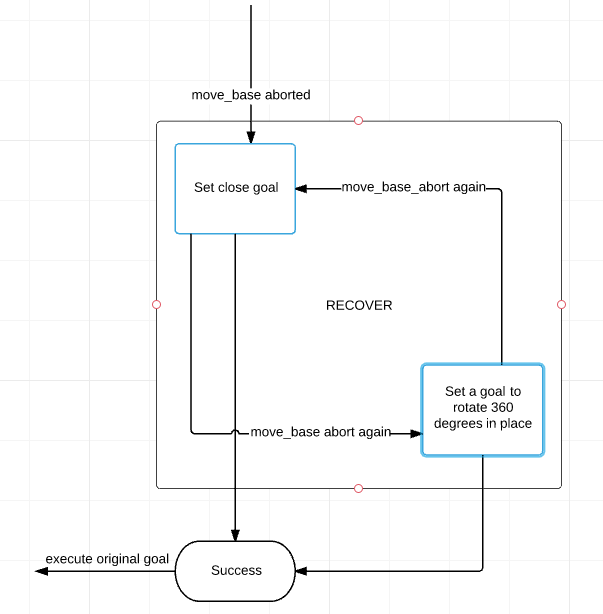
\includegraphics[width=26em]{Recovery.png} 
		\caption{SMACH中的简单恢复状态}
		%{Simple recovery state in SMACH}
	\end{center}
\end{figure}

\textbf{参数}:ROS的恢复行为的参数一般可以保留为默认值。为了清除代价地图进行恢复,你可以设置一个相对较高的模拟时间\mintinline{bash}{sim_time},这意味着轨迹很长,你可能需要考虑增加\mintinline{bash}{reset_distance}参数的值,这样可以消除本地代价地图上更大的区域,并且局部规划器有更好的机会寻找一条路径。

\section[Dynamic Reconfigure]{动态重新配置}%{Dynamic Reconfigure}

ROS导航最灵活的特性之一是动态重新配置,因为不同的参数设置可能对某些情况(如机器人靠近目标点时)更有帮助。即便如此,没有必要进行大量的动态重新配置。

\textbf{示例}:
我们在实验中观察到的一种情况是机器人常常会脱离全局路径,即使没有必要这么做或者这样做会带来不好的结果。
因此我们增加了路径距离偏差\mintinline{bash}{path_distance_bias}。由于大的路径距离偏差值\mintinline{bash}{path_distance_bias}将使机器人遵循全局路径,但实际上由于公差的原因机器人并不会最终到达目标点,我们需要一种方法让机器人毫不犹豫地达到目标点。
此时,我们动态减少路径距离偏差\mintinline{bash}{path_distance_bias},以便在机器人接近目标点时强调\mintinline{bash}{goal_distance_bias}。
毕竟,做更多的实验是为了找到解决问题的方法。

\section[Problems]{问题}%{Problems}

\begin{enumerate}
	\item 陷入困境。 %Getting stuck 	
	在使用ROS导航的时候,这个问题经常出现,无论是在仿真还是实际中,机器人都可能陷入困境然后放弃目标
	
	\item 不同方向采用不同的速度。%Different speed in different directions 
	在导航功能包中我们观察到一些奇怪的行为。当目标点设置在相对于TF原点的-x方向时,dwa局部规划器规划表现不稳定(局部规划的路径存在跳跃行为),而且机器人的移动速度非常缓慢。
	但是当把目标设置在+x方向时,dwa局部规划器就比较稳定了,并且移动速度很快。
	
	我在github上报告了这个问题:\url{https://github.com/ros-planning/navigation/issues/503}。目前还没有人尝试解决它。
	
	\item 实际VS.仿真。 %Reality VS. simulation 
	
	实际运行与仿真运行是有差别的。现实情况中,障碍物有各种各样的形状。例如,实验室有一个垂直的柜子,用以防止门关闭;由于柜子太细,机器人有时无法检测到柜子然后撞上柜子。而且实际中也会存在更复杂的人类活动。
	
	\item 不一致性。%Inconsistency 
	
	使用ROS导航功能包可能会出现不一致的行为。例如进门时,不同时间里局部规划器会一次又一次地生成差异较小的代价地图,这可能会影响路径规划,特别是在分辨率较低的时候。另外,机器人没有内存时,它不记得上次是怎么从门进入房间的,所以每次尝试进门都需要重新开始尝试。因此,如果机器人进门时采用与以前进门不同的角度,机器人可能会卡住并最终放弃目标。
	
\end{enumerate}


\section*{致谢}
希望本指南对你有所帮助。 请随意添加你在自己的实验中观察到的更多信息。
